% Numerical Computing II
% Homework 16
% Optimization
% February 20, 2010
% Problems 16.1,16.2,16.4 optional

\documentclass[11pt]{article}
\usepackage{listings}
\usepackage{graphicx}
\begin{document}         
% Start your text
\newcommand{\makehomework}[2]%
{\begin{center}%
	\Huge #1\\%
	\Large #2\\%
	Marty Fuhry\\%
	\today%
\end{center}}
\lstset{language=Matlab,numbers=left,frame=single,breaklines=true,morecomment=[l]{//}}
\makehomework{Numerical Computing II}{Homework 16: Optimization}

\section*{Exercise 16.1}
\lstinputlisting{problem_16_1.m}
Our endpoints after the fourth iteration of the Golden Section Search were:
	\begin{eqnarray*}
	a = 0.45835 \\
	b = 0.91670 \\
	\end{eqnarray*}
We find that the true max, $\pi/4$, is well between this interval. The estimated positions and values were as follows:
\begin{eqnarray*}
	x_l = 0.63343 \\ f(x_l) = 0.31417 \\
	x_r = 0.74163 \\ f(x_r) = 0.32167 \\
\end{eqnarray*}
These values very accurately approximate the max after only four iterations.
\pagebreak

\section*{Exercise 16.2}
\lstinputlisting{problem_16_2.m}

\pagebreak
The graph made by the fourth interpolating polynomial looks like this:

\begin{center}
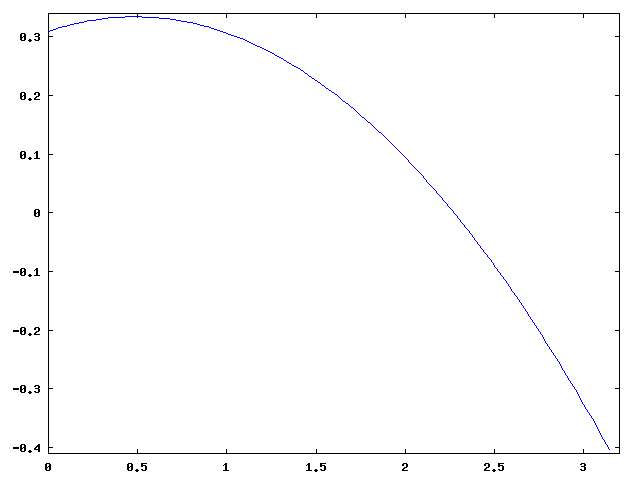
\includegraphics[scale=0.5]{problem_16_2.png}
\end{center}

This code interpolates a function quadratically in the least squares sense
using the endpoints $a$, $b$, and $x$. After interpolation, if the interpolated
polynomial has a maximum value, the first coefficient is negative. If the first
coefficient is not negative, then we can use the Golden Section Search to produce
a "close enough" approximation for a new value of $x$ to be used for our third
interpolation point. After each "successful" polynomial interpolation, the
furtheset point from the polynomial's max will be discarded.

Running this code, we receive values:
\begin{eqnarray*}
	x_m = .48300 \\ f(x_m) = 0.28653
\end{eqnarray*}

This is curiously no closer than the Golden Section Search. Though, after many
iterations, it does converge properly to the actual max value, $\pi/4$.

% Stop your text
\end{document}
